\documentclass[10pt,letterpaper]{article}

\usepackage{cogsci}
\usepackage{pslatex}
\usepackage{apacite}

\usepackage{amsmath, amsthm, amssymb}
\usepackage{graphicx}
\usepackage{color}

\newcommand{\TODO}[1]{\textcolor{red}{[TODO: #1]}}

\newcommand{\threshold}[0]{$T=2$}
\newcommand{\betazero}[0]{$\beta_0=683.86,\ 95\%\ \mathrm{CI}\ [601.66, 766.06]$}
\newcommand{\betaone}[0]{$\beta_1=46.01,\ 95\%\ \mathrm{CI}\ [19.71, 72.32]$}
\newcommand{\betatwo}[0]{$\beta_2=63.67,\ 95\%\ \mathrm{CI}\ [57.26, 70.07]$}
\newcommand{\kapb}[0]{$\kappa_b=50.42$}
\newcommand{\kapm}[0]{$\kappa_m=502850.41$}
\newcommand{\kapv}[0]{$\kappa_v=255.60$}
\newcommand{\perr}[0]{$\sigma_p=31.02$}
\newcommand{\sdzero}[0]{$\sigma_0=167.06$}
\newcommand{\sdadj}[0]{$\sigma_{adj}=0.9$}

\newcommand{\HoleResponseCorr}[0]{$r=0.77,\ 95\%\ \mathrm{CI}\ [0.75, 0.78]$}
\newcommand{\HoleRTCorr}[0]{$r=0.67,\ 95\%\ \mathrm{CI}\ [0.64, 0.71]$}
\newcommand{\PaddleCorr}[0]{$r=0.95,\ 95\%\ \mathrm{CI}\ [0.91, 0.97]$}

\newcommand{\AvgResponse}[0]{$53.2\%$}
\newcommand{\AvgCorrect}[0]{$72.4\%$}
\newcommand{\ResponseN}[0]{$N=15216$}
\newcommand{\AvgRT}[0]{$RT=1010.13\ \mathrm{msec},\ 95\%\ \mathrm{CI}\ [997.81, 1022.74]$}
\newcommand{\ResponseFull}[0]{$\chi^2(3)=64.469,p < 0.001$}
\newcommand{\ResponseHoleClass}[0]{$\chi^2(3)=4477.182,p < 0.001$}
\newcommand{\ResponseHoleSize}[0]{$\chi^2(1)=168.598,p < 0.001$}
\newcommand{\RTFull}[0]{$\chi^2(3)=27.146,p < 0.001$}
\newcommand{\RTHoleClass}[0]{$\chi^2(3)=63.611,p < 0.001$}
\newcommand{\RTHoleSize}[0]{$\chi^2(1)=8.981,p < 0.01$}
\newcommand{\RTZeroBounces}[0]{$RT=799.99\ \mathrm{msec},\ 95\%\ \mathrm{CI}\ [783.07, 815.99]$}
\newcommand{\InterceptZeroBounces}[0]{$\beta_0=757.86,\ 95\%\ \mathrm{CI}\ [756.67, 759.05]$}
\newcommand{\RTOneBounces}[0]{$RT=1027.87\ \mathrm{msec},\ 95\%\ \mathrm{CI}\ [1007.75, 1050.46]$}
\newcommand{\InterceptOneBounces}[0]{$\beta_0=894.24,\ 95\%\ \mathrm{CI}\ [891.74, 896.63]$}
\newcommand{\RTTwoBounces}[0]{$RT=1251.20\ \mathrm{msec},\ 95\%\ \mathrm{CI}\ [1225.41, 1276.81]$}
\newcommand{\InterceptTwoBounces}[0]{$\beta_0=1025.80,\ 95\%\ \mathrm{CI}\ [1021.74, 1029.79]$}


\title{Think again?\\ Optimal mental simulation tracks problem difficulty}

\author{{\large \bf Jessica B.~Hamrick$^1$ (jhamrick@berkeley.edu),
    Kevin A.~Smith$^2$ (k2smith@ucsd.edu),}\\
    {\large \bf Thomas L.~Griffiths$^1$ (tom\_griffiths@berkeley.edu),
      \& Edward Vul$^2$ (evul@ucsd.edu)}\\
    $^1$University of California, Berkeley, Department of Psychology, Berkeley CA 94720 USA\\
    $^2$University of California, San Diego, Department of Psychology, La Jolla, CA 92093 USA}

\begin{document}

\maketitle

\begin{abstract}
In this paper, we investigate the number of simulations that people run when reasoning about a task that requires mental simulation of physics. Specifically, we ask the question: do people vary the number of mental simulations that they run depending on the difficulty of the problem? And, if so, do they do so in a manner consistent with SPRT? To answer these questions, we ran a behavioral experiment in which people watched a ball bouncing around in a box, and had to judge whether it would first go through a hole in the wall, or bounce off that wall. We varied the difficulty of each trial by changing the size of the holes and the margin by which the ball either went through the hole or missed the hole. We hypothesized that people should be faster to respond on ``easy'' trials (e.g., where the ball goes directly through the center of a large hole, or hits the wall very far away from the hole), and slower to respond on ``hard'' trials (e.g., where the ball just barely goes through the hole, or just barely misses the hole). In brief, find that people's responses are well-predicted by a model of simulation, and that their response times are well-predicted by combining that model with a SPRT strategy. \TODO{this is identical to a paragraph in the introduction, and probably should be a little different at least}

\textbf{Keywords:} 
add your choice of indexing terms or keywords; kindly use a
semicolon; between each term
\end{abstract}

\section{Introduction}

%% The question we're interested in: how many simulations do people take?
Imagine you are playing a video game---for example, Angry Birds or Desert Golf---in which you need to predict where an object will end up. How do you know where to aim, and how long do you spend thinking about each shot before you take it? Recent research in the domain of intuitive physics and mental simulation has revealed that people make predictions like these by running noisy physical simulations \cite{Smith:2013fc,Battaglia2013,Smith:2013ug,Smith:2013th,Smith:2014tx,Ullman:2014ut,Hamrick:2015}. However, while this research has investigated the \emph{mechanism} by which people make these types of predictions, there has been very little investigation into \emph{how} people actually use this mechanism. If people are running mental simulations, \emph{how many} simulations do they run?

%% What's already been done
According to previous research by \citeA{Vul:2014ba}, a sample-based agent should only take a small number of samples before making a judgment---perhaps even just one. While taking a single sample is clearly suboptimal for each individual judgment, over the long run, taking a small number of samples maximizes expected utility across a large number of judgments. Does this story also hold true for mental simulations? There is some evidence that points to ``yes'': \citeA{Battaglia2013} analyzed the variability of people's responses in tasks concerning towers of building blocks, and found that participants seemed to use between three and seven samples per judgment.

A second question concerns the actual strategy used to take samples. Do people always take exactly the same number of samples for each decision, or do they vary the number of samples based on problem difficulty? While \citeA{Vul:2014ba} looked at a variety of strategies, they concluded that regardless of strategy, the optimal solution was still roughly the same: the agent should take very few samples. However, that does not make the choice of strategy irrelevant. If the strategy tells the agent to vary the number of samples, then we should see variability in the agent's response times. Indeed, such variability can be observed in other types of decision-making tasks, and has been well-modeled by the \textit{sequential probability ratio test} \cite{wald1947sequential}, or SPRT \cite<e.g.>{Gold:2007fo,Ratcliff:2008ux,Bitzer:2014ea}. In SPRT, the agent takes samples until it reaches a threshold number of samples in support of one hypothesis over another hypothesis.

\begin{figure*}[t]
    \begin{center}
        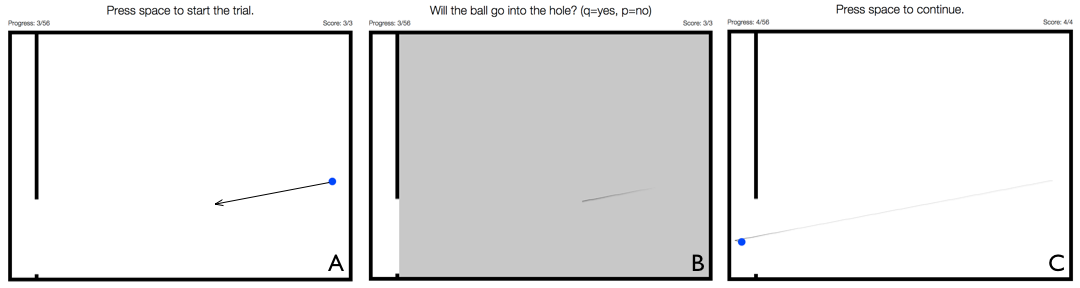
\includegraphics[width=\textwidth]{figures/experiment.png}
        \caption{\textbf{Example experimental trial.} Each panel shows a different part of the trial. The left panel shows the initial screen presented to the participant. The middle panel shows the occluded ball, after observing the stimulus presentation. The faded gray line shows the path the ball took during the initial presentation. The right panel shows the final position of the ball, after observing the feedback. As in the middle panel, the faded gray line shows the path of the ball.}
        \label{fig:experiment}
    \end{center}
\end{figure*}

%% What we're going to do and how we're going to do it
In this paper, we investigate the number of simulations that people run when reasoning about a task that requires mental simulation of physics. Specifically, we ask the question: do people vary the number of mental simulations that they run depending on the difficulty of the problem? And, if so, do they do so in a manner consistent with SPRT? To answer these questions, we ran a behavioral experiment in which people watched a ball bouncing around in a box, and had to judge whether it would first go through a hole in the wall, or bounce off that wall. We varied the difficulty of each trial by changing the size of the holes and the margin by which the ball either went through the hole or missed the hole. We hypothesized that people should be faster to respond on ``easy'' trials (e.g., where the ball goes directly through the center of a large hole, or hits the wall very far away from the hole), and slower to respond on ``hard'' trials (e.g., where the ball just barely goes through the hole, or just barely misses the hole). In brief, find that people's responses are well-predicted by a model of simulation, and that their response times are well-predicted by combining that model with a SPRT strategy.

%% Plan of the paper
The plan of the paper is as follows. First, we describe an experiment in which we asked participants to respond to the question of, ``will the ball go through the hole?'', and analyze people's accuracy and response times. Second, we formalize our hypothesis of how people make judgments in this experiment by specifying a combination of a simulation-based model with the SPRT strategy. Third, we describe a second experiment based on the experiment from \citeA{Smith:2013fc} that was used to fit the parameters of our model. Then, we compare the model's predictions to people's responses in Experiment 1. Finally, we discuss the implications of our results on the broader, underlying question: how do people use mental simulation?

\section{Experiment 1: Will the ball go in the hole?}

\begin{figure*}[t]
    \begin{center}
        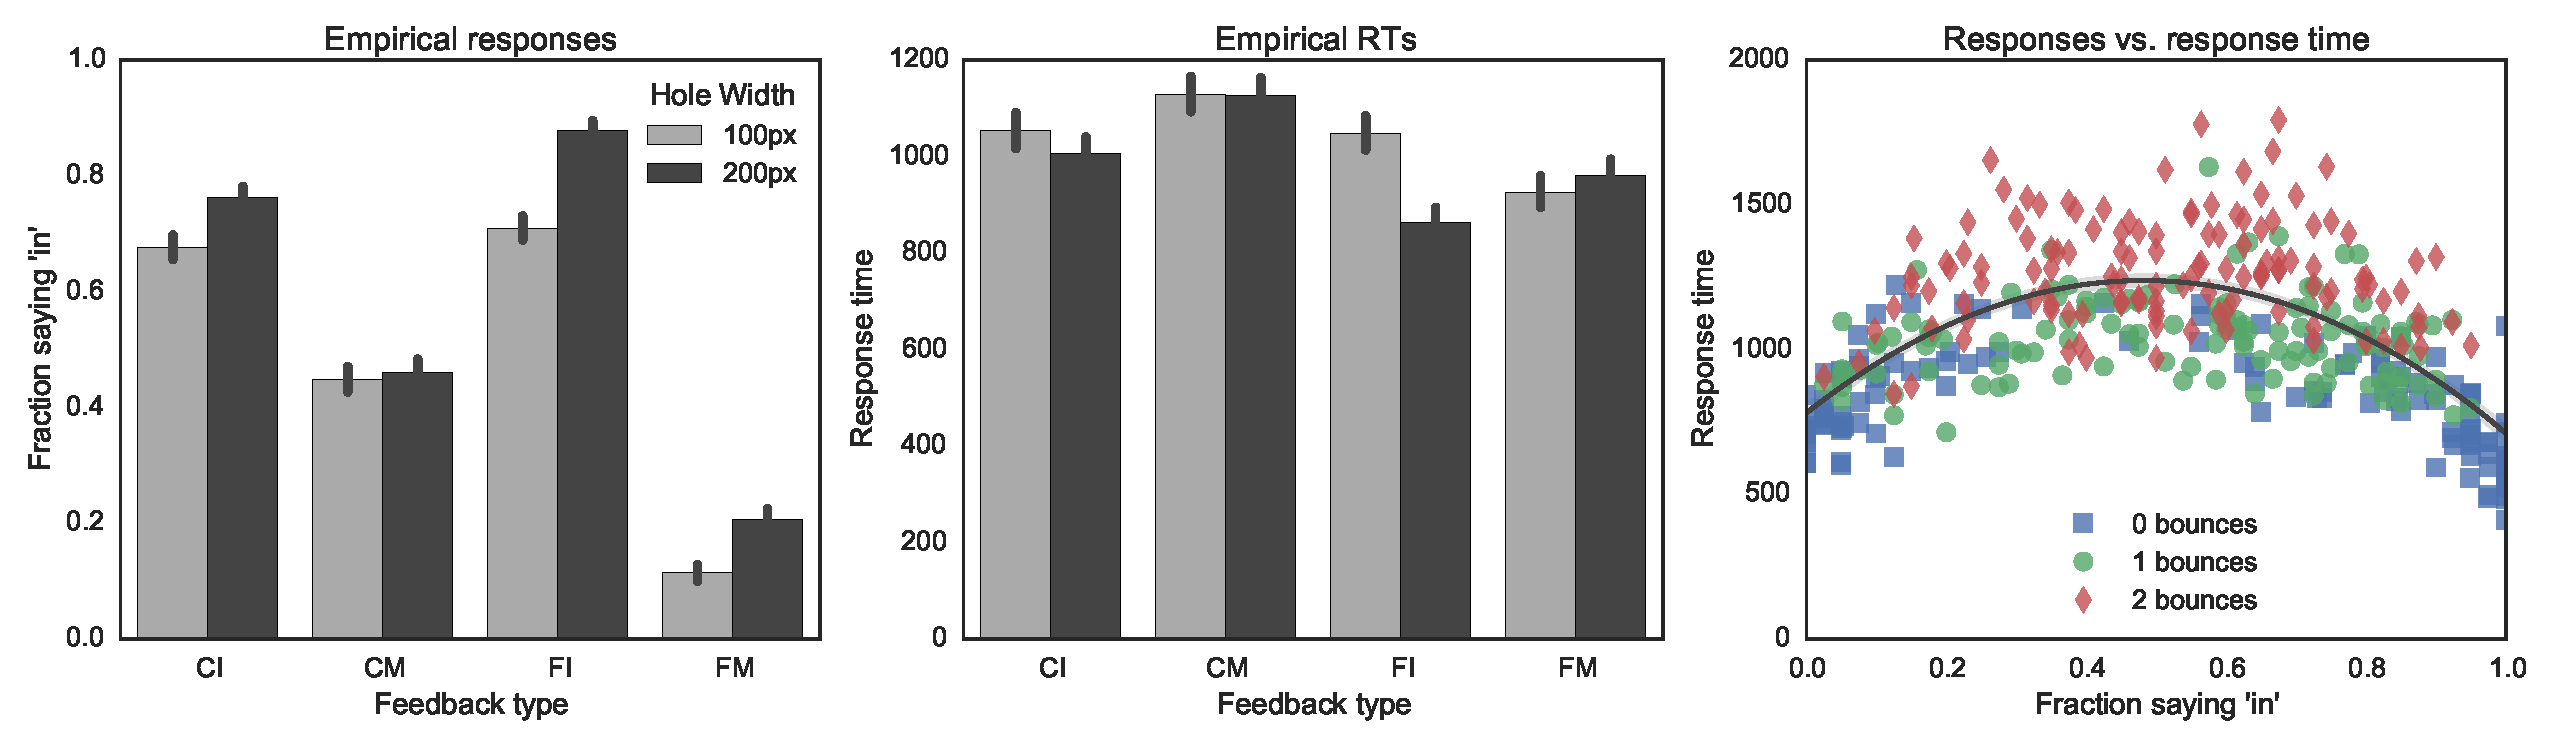
\includegraphics[width=\textwidth]{figures/hole_empirical_results.pdf}
        \caption{\textbf{Response times as a function of response.} Left subplot: each bar shows the proportion of participants saying that the ball will go in the hole for a particular feedback type ($x$-axis) and hole size (color). Middle subplot: like the left subplot, but the $y$-axis shows bootstrapped logarithmic means of response times. Right subplot: each point corresponds to a different stimulus, feedback type, and hole size.  The $x$-axis is the proportion of participants saying the ball will go in the hole, and the $y$ axis is the logarithmic mean response time.}
        \label{fig:pct-vs-rt}
    \end{center}
\end{figure*}

In order to determine whether people take multiples samples---and if they vary the number of samples---we designed an experiment in which people had to determine whether a ball would go into a hole (see Figure \ref{fig:experiment}). In particular, we designed the trials in this experiment such that some were harder than others.

\subsection{Participants}

We recruited $N=328$ participants on Amazon's Mechanical Turk using the psiTurk \cite{McDonnell12} experimental framework. Participants were treated in accordance with UC Berkeley IRB standards and were paid \$0.60 for approximately 6.5 minutes of work. Participants were randomly assigned to one of eight conditions, which determined which stimuli they judged based on a latin-square design (see Stimuli). Additionally, we excluded $N=8$ participants from analysis for answering incorrectly on more than one control trial (see Stimuli), leaving a total of $N=320$ participants.

\subsection{Stimuli}

The stimuli consisted of animations depicting a blue ball with a radius of 10px bouncing around in a box with dimensions 900px $\times$ 650px. All stimuli consisted of two separate animations. The first was the stimulus presentation, which had a duration of 0.775 seconds and depicted the ball moving in a particular direction. The second animation was the feedback, which picked up immediately where the first animation left off, and which had a duration of 1.5 seconds and depicted the ball either going into the hole or bouncing off the wall that contained the hole.\footnote{To enforce the constraint that the ball always travel the same distance during the feedback animation, the $x$-coordinate of the wall with the hole in it was allowed to vary across stimuli.} During the feedback animation, the ball could bounce on the other walls either 0, 1, or 2 times before going into the hole hitting the wall with the hole in it. In both animations, the ball had a velocity of 400px/s. Additionally, in the animations, the path that the ball had traveled so far was drawn with a faded gray line (see Figure \ref{fig:experiment}).

There were 48 different initial animations, and for each of these intial animations, there were four different types of feedback and two different hole sizes, giving a total of eight versions of each stimulus. The four feedback types were: ``far in'' (FI), where the ball went directly through the center of the hole; ``far miss'' (FM), where the ball missed the hole by a wide margin; ``close in'' (CI), where the ball just barely went through the hole; and `` close miss'' (CM), where the ball just barely missed the hole. The two hole sizes were 100px and 200px.

In order to ensure that participants never saw the same initial animation twice, we used a latin-square design of Initial Animation $\times$ Hole Type $\times$ Hole Size. Thus, each participant saw each initial animation exactly once, each hole type exactly 12 times, and each hole size exactly 24 times.

In addition to the 48 experimental trials, there were seven instruction trials and eight control trials, which were the same for all participants. The control trials were designed to be extremely easy and were either of type ``straight hit'' (with a hole size of either 300px or 350px) or ``far miss'' (with a hole size of 100px). Thus, participants saw a total of 63 trials throughout the experiment.

\subsection{Procedure}

The experiment was divided into two phases: the training phase, and the experimental phase. During the training phase, participants made judgments on the seven instruction trials in order to get used to the task. During the experimental phase, participants made judgements on the 48 experimental trials, presented in a random order, as well as the eight control trials, which were also shown in a random order, but interspersed with the experimental trials such that every 8th trial was a control trial.

On each trial, participants were shown the scene, including the initial position of the ball and the location of the hole. Participants were instructed to press the ``space'' key to begin the trial. Immediately upon pressing ``space'', the initial stimulus presentation began. As soon as the initial stimulus animation concluded, a gray box was drawn over the screen, occluding the ball (but not the line depicting the path it had traveled so far; this was left in as a reminder to participants of where the ball had come from). Participants were asked, ``will the ball go in the hole?'', and were instructed to press `q' to respond in the affirmative, and `p' to respond in the negative. Immediately after responding, text appeared saying ``Correct!'' or ``Incorrect.'', depending on the participants' response. Additionally, the gray occluder was removed, and participants were shown the feedback animation. After the feedback animation was complete, the final frame of the animation remained on the screen until participants pressed ``space'' to advance to the next trial. 

Throughout the experiment, participants saw two counters: one showing their total progress (the number of trials completed / total trials), and their score (the number of times they answered correctly / the number of trials completed).

\subsection{Results}

\subsubsection{Responses}

On average, participants were correct \AvgCorrect{} of the time and responded that the ball would go in the hole \AvgResponse{} of the time (\ResponseN{}), excluding catch trials. There was a significant effect of feedback type on participants' responses (\ResponseHoleClass{}) as well as a significant effect of hole size (\ResponseHoleSize{}). Additionally, there was an interaction between feedback type and hole size (\ResponseFull{}). Figure \ref{fig:pct-vs-rt} (left subplot) shows responses as a function of feedback type and hole size.

\subsubsection{Response times}

For all analyses of response time, we computed averages using bootstrapped logarithmic means (exponential of the mean of the log response times), using 1000 bootstrap samples. Participants had an average response time of \AvgRT{} milliseconds (\StdRT{}ms), excluding catch trials. There were significant effects of both feedback type (\RTHoleClass{}) and hole size (\RTHoleSize{}) on response time, as well as an interaction between feedback type and hole size (\RTFull{}). However, the hole size was only significant in the case of the ``far in'' (FI) trials ($p<0.001$), in which the ball went straight through the center of the hole. Figure \ref{fig:pct-vs-rt} (middle subplot) shows the response times as a function of feedback type and hole size.

\subsubsection{Relationship of responses to reaction time}

As shown in Figure \ref{fig:pct-vs-rt} (right subplot), we found a clear effect of certainty on people's response times. In particular, participants were on average faster to respond on trials that they were more certain about, and slower to respond to trials that they were unsure about. This tradeoff mirrors the same tradeoff found in SPRT: decisions for which $p\approx0.5$ are slower, because it takes longer to get to one threshold versus the other. Thus, it is clear that people are not spending a fixed amount of time thinking about each trial; rather, they spend more time thinking about the ``hard'' trials than the ``easy'' trials.

\section{Modeling mental simulations}

How do people make the types of judgments that they did in Experiment 1? We hypothesized that they predict where the ball will go by running noisy physical simulations, and that they run a variable number of simulations on each trial according to the \textit{sequential probability ratio test}, or SPRT \cite{wald1947sequential}. In this section, we lay out the formalism for both the simulation-based model and the SPRT strategy.

\subsection{The ``Noisy Newton'' hypothesis}

There is a growing body of evidence that people reason about physical scenes by running noisy simulations. This hypothesis, referred to as the ``Noisy Newton'' hypothesis, states that people have approximate knowledge of physical laws instantiated in a runnable model of intuitive physics. Using this model, they can extrapolate the future of physical scenes by running a series of noisy simulations \cite{Smith:2013fc,Battaglia2013,Smith:2013ug,Smith:2013th,Smith:2014tx,Ullman:2014ut,Hamrick:2015}. In particular, \citeA{Smith:2013fc} investigated the various sources of uncertainty in these simulations, finding that people's judgments were best captured by a model that took into account both perceptual uncertainty and dynamics uncertainty.

Specifically, \citeA{Smith:2013fc} asked people to catch a ball like the one in Figure \ref{fig:experiment} using a paddle that could move up and down along the $y$-axis. In order to predict where people would place the paddle on each trial, their model incorporated uncertainty in its physical simulations through five parameters: perceptual uncertainty over the position of the ball ($\sigma_p$), uncertainty in the initial direction of velocity ($\kappa_v$), ongoing uncertainty in the direction of movement ($\kappa_m$), uncertainty in the bounce angle ($\kappa_b$), and a ``center bias'' reflecting a bias for people to respond more towards the center of the $y$-axis ($\sigma_0$).

\subsection{The SPRT strategy}

In this paper, we consider binary (or two-alternative forced choice) decisions, where an agent must choose one of two hypotheses, $H_0$ or $H_1$. The agent may take samples $X_i$ from a Bernoulli distribution parameterized by an unknown parameter $p$, and from these samples estimate $\hat{p}=\frac{1}{N}\sum_{i=1}^N X_i$, where $N$ is the total number of samples. Then, the decision rule which minimizes the probability of error is $\hat{H}(X_1,\ldots{},X_N)=H_0$ when $\hat{p}<0.5$ and $\hat{H}(X_1,\ldots{},X_N)=H_1$ when $\hat{p}>0.5$.

In the best possible case, the agent takes infinite samples and chooses the maximum \emph{a posteriori} (MAP) hypothesis with probability $p$. In practice, the agent cannot take infinite samples. Thus, to determine when to stop sampling (i.e., what the value of $N$ is), we use the \emph{sequential probability ratio test} \cite{wald1947sequential}. When using a SPRT strategy, the agent accumulates $Y_N=\sum_{i=1}^N 2X_i-1$, and stops either when $Y_N=T$ or $Y_N=-T$, for some threshold number of samples $T$. 

\subsubsection{Modeling responses} Independent of the number of samples actually taken, the probability of choosing $H_1$ given that $H_1$ is the MAP hypothesis is:
\begin{equation}
\Pr[\hat{H}(Y_N)=H_1\,|\,H_1]=\frac{p^T}{p^T+(1-p)^T},
\label{eq:pr-choose-h1}
\end{equation}

We can compute the probability, $p$, that the ball goes in the hole by running simulations from the model.

\subsubsection{Modeling response times} Given the threshold, the probability of taking $N$ samples and then choosing $H_1$ is:
\begin{multline}
\Pr[N,H_1\,|\,T,p]=\left(\frac{2^N}{2T}\right)p^{\frac{N+T}{2}}(1-p)^{\frac{N-T}{2}}\cdot{}\\
\sum_{\nu=1}^{2T-1}\cos\left(\frac{\nu\pi}{2T}\right)^{N-1}\sin\left(\frac{\nu\pi}{2T}\right)\sin\left(\frac{\nu\pi}{2}\right)
\end{multline}
for $N\geq T$ and where $N$ is of the same parity as $T$ \cite[ch.~XIV, eq. 5.7]{Feller:1968ut}. Because we are dealing with binary hypotheses, the marginal probability of $N$ samples is then:
\begin{equation}
\Pr[N\,|\,T,p]=\Pr[N,H_1\,|\,T,p]+\Pr[N,H_1\,|\,T,1-p].
\label{eq:pr-n}
\end{equation}
and so the expected number of samples for a particular decision is:
\begin{equation}
\mathbb{E}[N\,|\,T,p]=\sum_{N=T}^\infty N\cdot{}\Pr[N\,|\,T,p]
\end{equation}

Assuming every sample takes the same amount of time, response times as predicted by the model should be directly proportional to $\mathbb{E}[N\,|\,T,p]$. However, we found the number of bounces to be an extremely strong predictor of response time in Experiment 1: each additional bounce adds a constant amount of time to the response. To account for this, our final response time equation incorporated the number of bounces, $B$, as follows:
\begin{equation}
t = \beta_0 + (\beta_1 + \beta_2\cdot{}\mathbb{E}[B]) \cdot{}\mathbb{E}[N\,|\,T,p]
\label{eq:rt}
\end{equation}
where $\beta_0$, $\beta_1$, and $\beta_2$ are fitted coefficients.

\section{Experiment 2}

Based on the results of Experiment 1, it is clear that people are spending longer on decisions that they are less confident about. In order to determine whether this could be explained by running mental simulations according to the SPRT strategy, we first needed to better characterize the parameters of people's mental simulations. Experiment 2 was designed as a conceptual replication of \citeA{Smith:2013fc}, which would allow us to affirm that people are using mental simulation on these types of tasks, and if so, what the parameters of those simulations are.

\subsection{Participants}

We recruited $N=60$ participants on Amazon's Mechanical Turk using the psiTurk \cite{McDonnell12} experimental framework. Participants were treated in accordance with UC Berkeley IRB standards and were paid \$0.60 for approximately 5 minutes of work. Additionally, we excluded $N=18$ participants from analysis for failing to catch the ball on more than one control trial, leaving a total of $N=42$ participants.

\subsection{Stimuli}

The stimuli were modified versions of those used Experiment 1, with two major differences. First, instead of a wall with a hole in it, there was a paddle of length 100px that could move up and down the $y$-axis. Second, there was no feedback animation; instead, there was just a single feedback image corresponding to the last frame of the feedback animation. Because there was no feedback animation, there were only 48 stimuli (corresponding to the stimulus presentation animations from Experiment 1), plus the seven instruction trials and eight catch trials.

\subsection{Procedure}

Like Experiment 1, the experiment was divided into two phases: the training phase (consisting of seven trials), and the experimental phase (consisting of the 48 experimental trials, with the eight control trials evenly interspersed). On each trial, participants were shown the scene, including the initial position of the ball and the location of the hole. The paddle begin at the center of the $y$-axis, and was freely moveable along the $y$-axis from the very beginning of the trial. Participants were instructed to press the ``space'' key to begin the trial. 

As in Experiment 1, immediately upon pressing ``space'', the initial stimulus presentation began, after which an occluder appeared. However, unlike Experiment 1, as soon as the occluder appeared, a timer also appeared and begin counting down for 2 seconds. During this time, participants had to move the paddle to try to catch the ball in the position it would be when the timer was up.When the timer countdown finished, the paddle froze at its current location, and the occluder was removed and the full path of the ball revealed. If the ball was on the paddle, then participants were told, ``You caught the ball!''. If the ball was not on the paddle, participants were told ``Oops, you didn't catch the ball.'' Participants were then instructed to press ``space'' to continue, at which point the next trial would begin.

Throughout the experiment, participants saw two counters: one showing their total progress (the number of trials completed / total trials), and their score (the number of times they caught the ball / the number of trials completed).

\section{Results}

\begin{figure*}[t]
    \begin{center}
        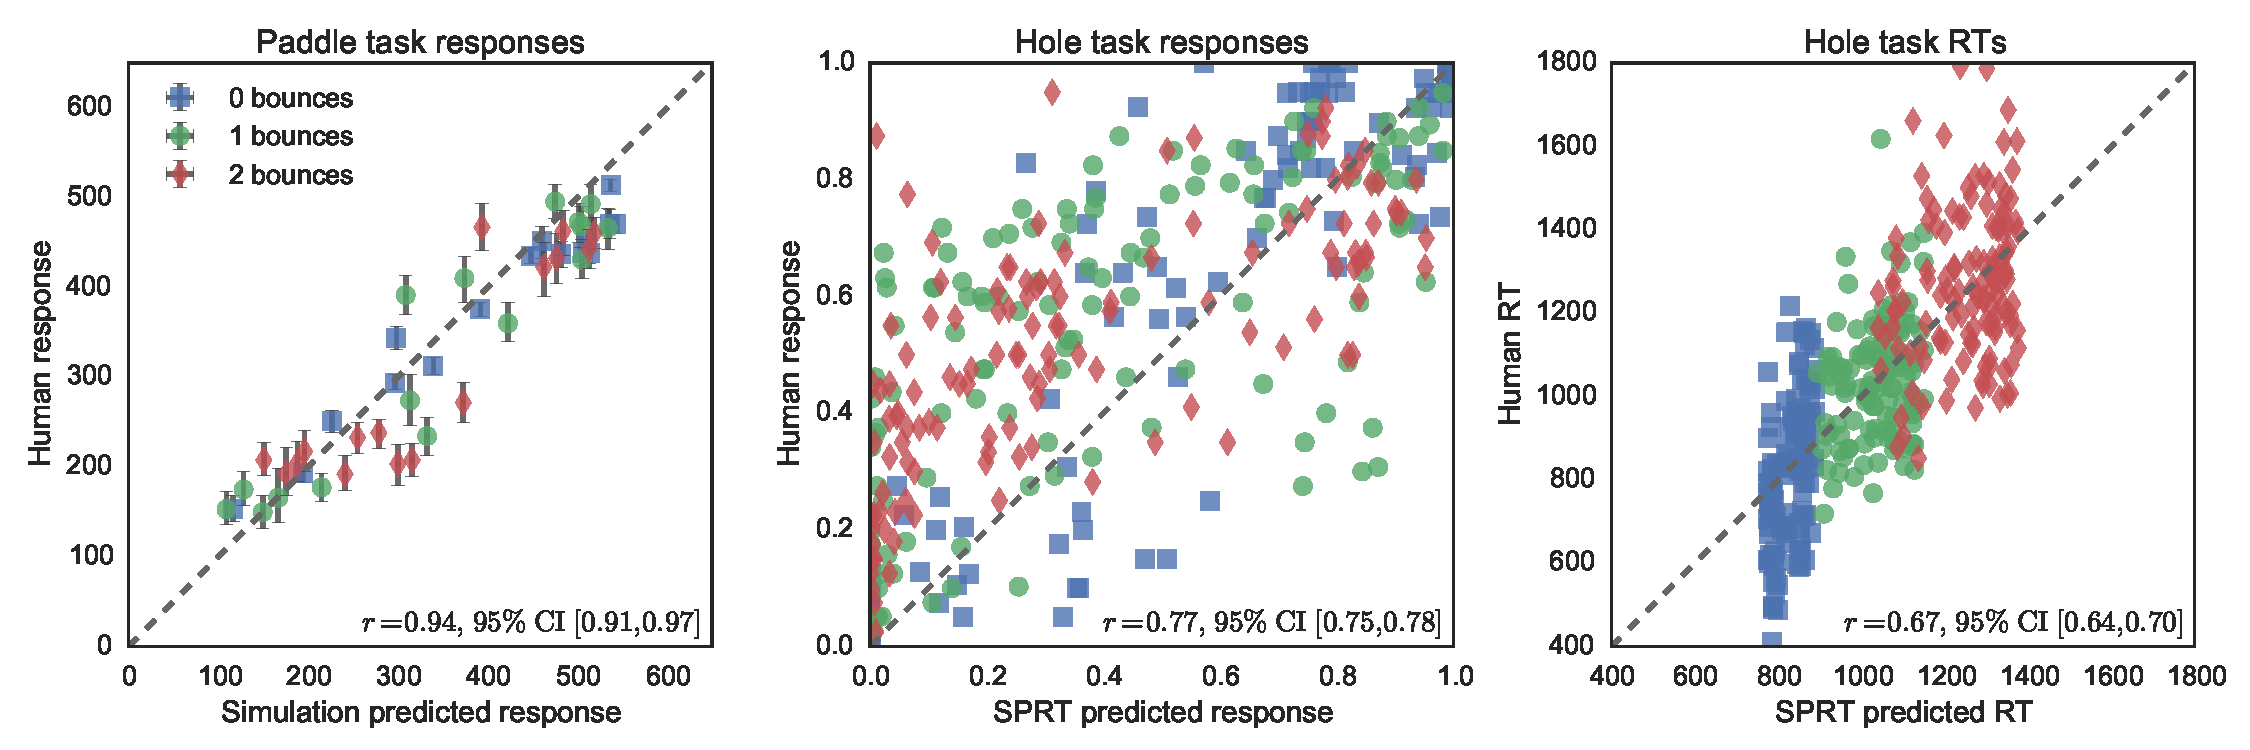
\includegraphics[width=\textwidth]{figures/model_results.pdf}
        \caption{\textbf{Model vs. human judgments in the paddle task.} \TODO{}}
        \label{fig:model-results}
    \end{center}
\end{figure*}

We fit the model to people's responses in two steps. First, we fit $\sigma_p$, $\kappa_v$, $\kappa_m$, $\kappa_b$, and $\sigma_0$ to particant's responses in Experiment 2 \cite<for details, see>{Smith:2013fc}. Using this procedure, we found the best fitting parameters to be \perr{}, \kapv{}, \kapm{}, \kapb{}, and \sdzero{}. With these parameters, we find very similar results to those from \citeA{Smith:2013fc} (Figure \ref{fig:model-results}, left subplot). In particular, we found a correlation of \PaddleCorr{} between the model's predicted means of where the ball would end up and people's average location of the paddle.

From the fitted model, we can estimate the probability that the ball goes in the hole ($p$), with one adjustment. Specifically, it is not clear how many samples people take to solve the paddle task. If they are taking a fixed number of samples, $M$,\footnote{We assume that in the paddle experiment, people are taking a fixed number of samples, as they only have a small, fixed amount of time to respond.} then we can estimate the true standard deviation of their simulations as $\sigma_{sims} = \sigma_{judgments} / \sqrt{M}$. As $M$ is unknown, we treat it as an additional free parameter in our model, adjusting the standard deviation of the model's responses by a fixed constant, $\sigma_{adj}=\sqrt{M}$.

We fit $\sigma_{adj}$ and $T$ using a grid search to maximize the correlation between SPRT response times (Equation \ref{eq:rt}) and actual response times in Experiment 1. To compute Equation \ref{eq:rt}, we ran $n=10000$ samples from the model, and from these samples (as well as the $\sigma_{adj}$ adjustment) estimated a truncated normal distribution along the wall with the hole in it. From this truncated normal, we computed the value of $p$ as the the probability density lying within the region of the hole. From this procedure, we found the best fitting parameters to be \sdadj{} and \threshold{}.\footnote{If \sdadj{}, then $M<1$. How could people be taking fewer than one sample? We suspect that $\sigma_{adj}<1$ because the model actually overestimates the standard deviation; thus, $\sigma_{adj}$ is adjusting for both the inflated uncertainty in the model as well increased certainty in people's judgments on the paddle task.}

Finally, we fit the coefficients from Equation \ref{eq:rt} to people's responses in Experiment 1 using an ordinary least squares regression, where $\mathbb{E}[B]$ and $\mathbb{E}[N\,|\,T,p]$ were computed directly from model simulations. The best-fitting parameters were \betazero{}, which corresponded to the intercept; \betaone{}, which corresponded to the number of samples before making a decision; and \betatwo{}, which corresponded to the number of bounces before making a decision.

Participant responses were well correlated with a SPRT model with \threshold{} (\HoleResponseCorr{}). There was also a significant correlation with resonse time for the \threshold{} SPRT model as computed with Equation \ref{eq:rt} (\HoleRTCorr{}). Figure \ref{fig:model-results} shows human responses as a function of the model's responses for \threshold{} (middle subplot) as well as human response times as a function of the model's response times (right subplot).

\section{Discussion}

In this paper, we asked the question: how many simulations do people run? We hypothesized that although people probably take a very small number of samples \cite{Vul:2014ba}, people still vary the number of samples that they take in order to exploit the fact that some judgments are easier to make than others. Specifically, we hypothesized that people take samples in a manner consistent with the SPRT strategy, in which evidence for hypotheses is accumulated until one hypothesis has a fixed amount of evidence over the other.

The results of Experiment 1 paint a clear picture that people \emph{do} vary the number of samples they take, as evidenced by the increase in response time on ``hard'' trials (i.e., trials which people are less confident about). This pattern of taking longer to respond on trials with $p\approx 0.5$ is qualitatively consistent with the strategy of SPRT. To demonstrate quantitatively that SPRT is a good account for people's responses, we formulated a model of people's responses based on the ``Noisy Newton'' hypothesis and SPRT. In Experiment 2, replicated the experiment from \citeA{Smith:2013fc}, and used the results to fit our model. Comparing people's responses and response times in Experiment 1 to those of the model, we found an extremely strong fit, suggesting that people are relying both on simulations from approximate physical simulations, and that they vary the number of simulations that they run according to SPRT.

\bibliographystyle{apacite}

\setlength{\bibleftmargin}{.125in}
\setlength{\bibindent}{-\bibleftmargin}

\bibliography{references}

\end{document}
